\section{Experiments} \label{sec:experiments}

As a first impression, it is a good idea to use planning in both of
these domains.  In the GIVE domain, SGPLAN 5.2.2 computes a domain
plan from the initial state to the goal in 0.3 seconds, which is fast
enough for the application.\footnote{All reported runtimes were
  measured on a Pentium 4 CPU running at 3 GHz. Java programs were allowed
  to ``warm up'', i.e.\ the planner was run five times in a row and the
  first four measurements discarded to ensure that the JVM had just-in-time
  compiled all relevant bytecode.}  In the sentence
generation domain, FF dramatically outperforms the best previously known
algorithm for the same problem (a reimplementation of \cite{Stone2003a}),
although the latter is a greedy search algorithm with a heuristic that is
hand-tailored to the domain.

However, we also observed that although FF manages the search for a
plan very efficiently, it spends comparatively large amounts of time
on computing instances, most of which are then never used during the
search.  Below, we report on a series of experiments that are designed
to improve our understanding of this situation.

\subsection{Experiment 1: Sentence generation}
\label{sec:exper-1:-sent}

For the first experiment, we generated a series of sentence generation
problems which required the planner to compute a plan representing the
sentence ``Mary likes the Adj$_1$ \ldots Adj$_n$ rabbit.''  Each
problem instance assumed a certain number $m$ of rabbits that were
distinguished by $n \leq m$ different properties, such that all $n$
properties were required to distinguish the target referent from all
other rabbits.  The $n$ properties are realized as $n$ different
adjectives, in any order.  This setup allows us to control the plan
length (a plan using $n$ properties will have length $n+4$) and the
universe size (the universe will contain $m+1$ individuals in addition
to the differently-typed individuals for encoding the grammar).

\begin{figure}
  \centering
  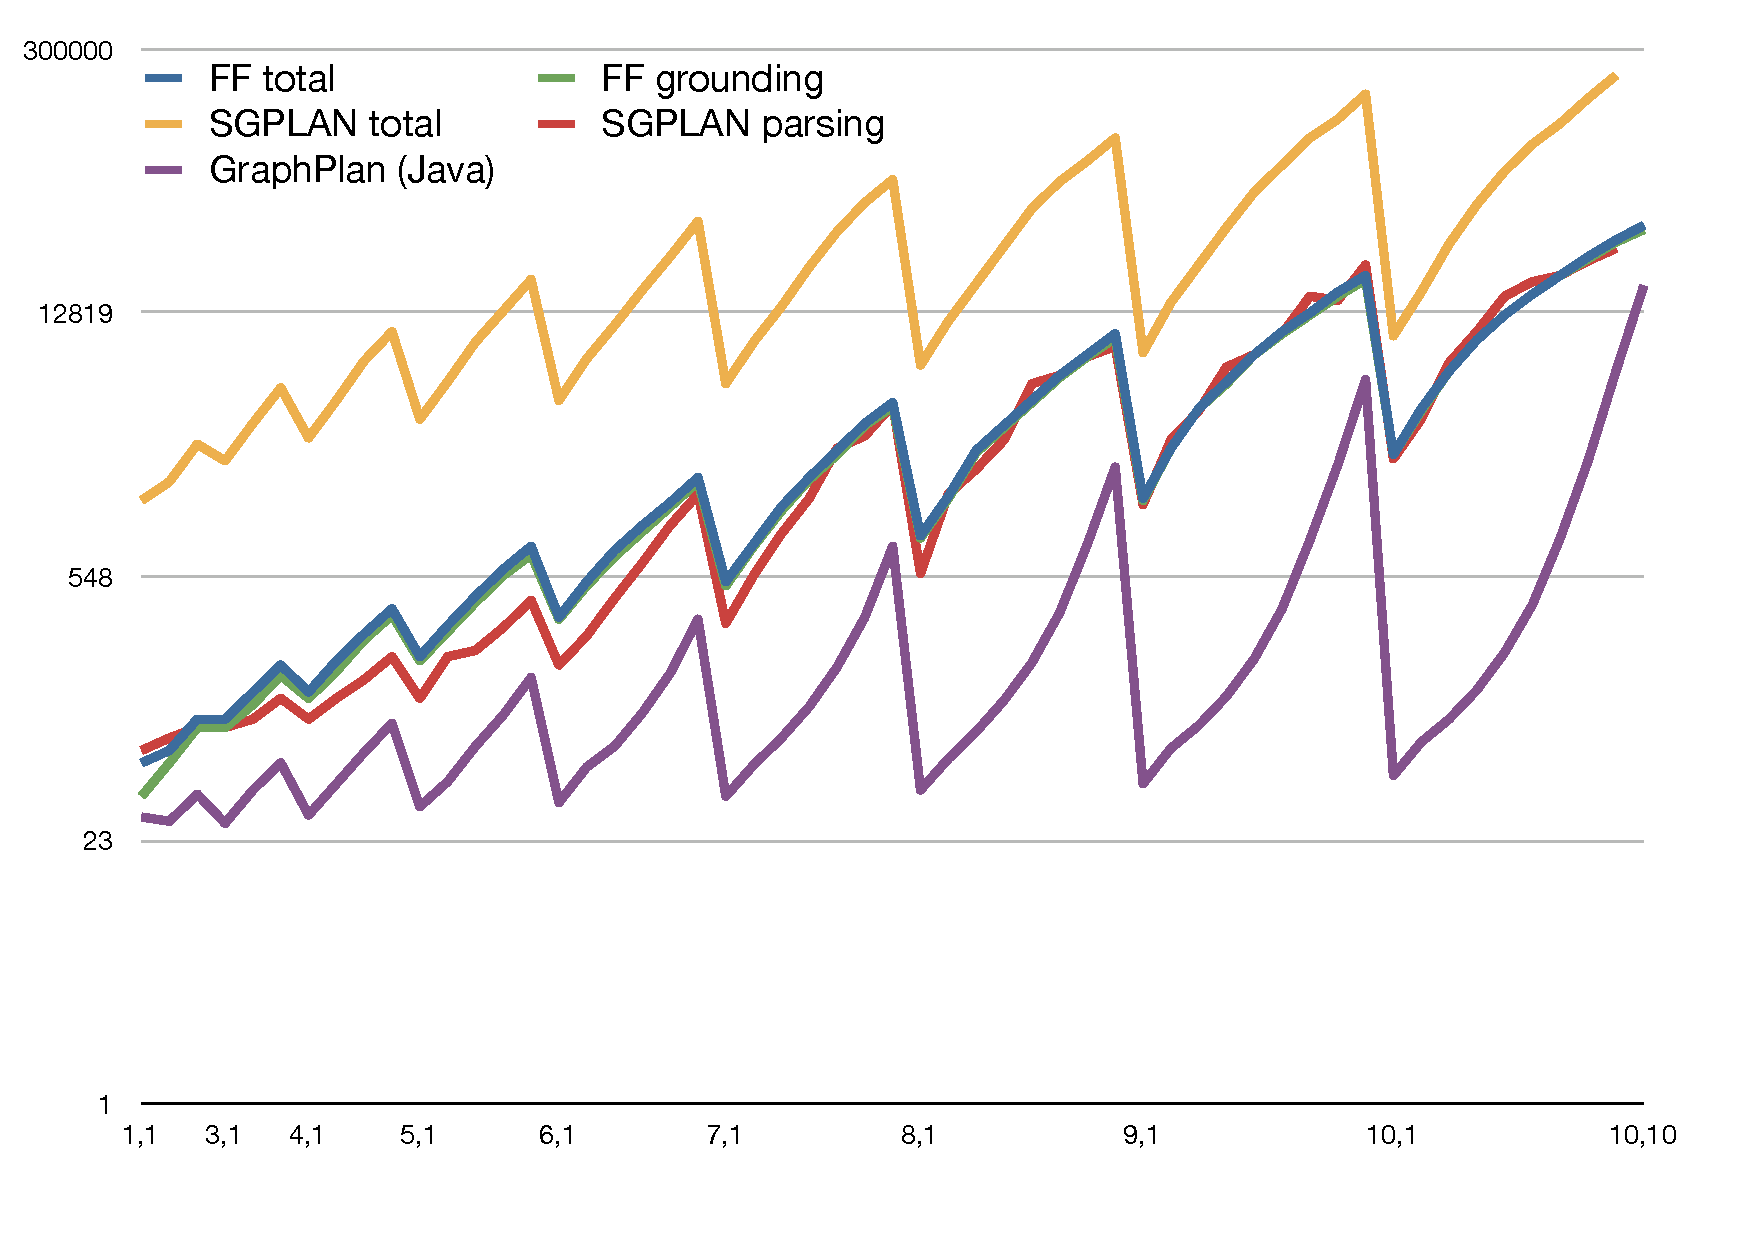
\includegraphics[width=1\columnwidth]{pic-runtime-modifiers-with-sgplan}
  \caption{Runtimes in the sentence generation domain.  The horizontal
  axis represents parameters $(m,n)$ from $(1,1)$ to $(10,10)$ in
  lexicographical order.}
  \label{fig:runtimes-crisp}
\end{figure}

The results of this experiment are shown in
Fig.~\ref{fig:runtimes-crisp}; we plot the input parameters $(m,n)$
(in lexicographic order) on the horizontal axis and the runtime in
milliseconds on the vertical axis.  The figure reveals a number of
interesting insights.  First of all, FF significantly outperforms
SGPLAN in this domain.\footnote{Experiments with SGPLAN were run with
  a pre-release version of SGPLAN that was kindly provided by Chih-Wei
  Hsu, as the release version of SGPLAN 5.2.2 has a bug which causes
  it to crash on some instances.}  Second, FF's runtime is dominated
by its initial grounding step, in which it computes the ground
instances of all predicates and actions used in the planning problem
to avoid unification during search: The ratio of grounding time to
total runtime is generally above 85\%, and rises above 99\% at $m=11$,
which is still a small universe in this application.\footnote{The
  ``grounding'' time reported here is what FF reports as ``time spent:
  instantiating action templates''.}  This is also reflected in the
much higher sensitivity of FF to the domain size: If we fix $n=1$, FF
takes 60 ms to compute a plan at $m=1$, but 2.4 seconds at $m=10$; by
contrast, our GraphPlan implementation takes 30 ms at $m=1$ and still
only 50 ms at $m=10$.

As a consequence, even FF is outperformed quite clearly by an ad-hoc
Java implementation of GraphPlan which only computes instances of
predicates and actions as they are discovered while the planning graph
gets built.  On the other hand, the runtime that FF actually spends on
search is again considerably lower than that of our GraphPlan
implementation, and for any given $m$, GraphPlan's runtime grows much
faster with $n$ (i.e.\ the plan size) than FF's.  We conclude that on
the sentence planning domain, FF does very well on search, but then
spends about ten times as much runtime again on grounding.



\subsection{Experiment 2: Minimal GIVE worlds}
\label{sec:exper-2:-minim}

To evaluate the performance of the planners on the planning problems
that arise in the GIVE domain, we construct a sequence of test worlds
as illustrated in Fig.~\ref{fig:give-minimal}.  These worlds consist
of a $2n$ by $h$ grid of positions, such that there are buttons at
positions $(2i-1,1)$ and $(2i,h)$ for $1 \leq i \leq n$.  The player
starts in position $(1,1)$ and must press all buttons in order to
complete the game.  The world is generated as a GIVE world
description, and then converted into a planning problem by the GIVE
software. \todo{at what level of detail should we describe this?}

\begin{figure}
  \centering
  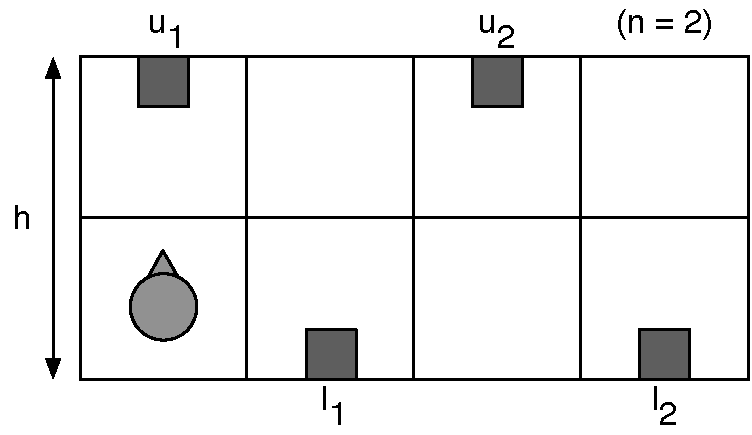
\includegraphics[width=1\columnwidth]{pic-buttons}
  \caption{Minimal GIVE world.}
  \label{fig:give-minimal}
\end{figure}

Some results from this experiment (for $h=20$, with $n$ ranging from
$1$ to $40$) are shown in Fig.~\ref{fig:give-runtime-minimal}.  The
most obvious result is that FF is unable to solve any problems beyond
$n=13$ on the experimentation machine within the memory limit of 1 GB.
SGPLAN, on the other hand, solves instances beyond $n=40$ without
major problems.  The time spent on grounding is not a major factor in
either planner, probably because the planners need more time to
actually compute the plan -- at $n=40$, the optimal plan has a length
of about 1600!

\begin{figure}
  \centering
  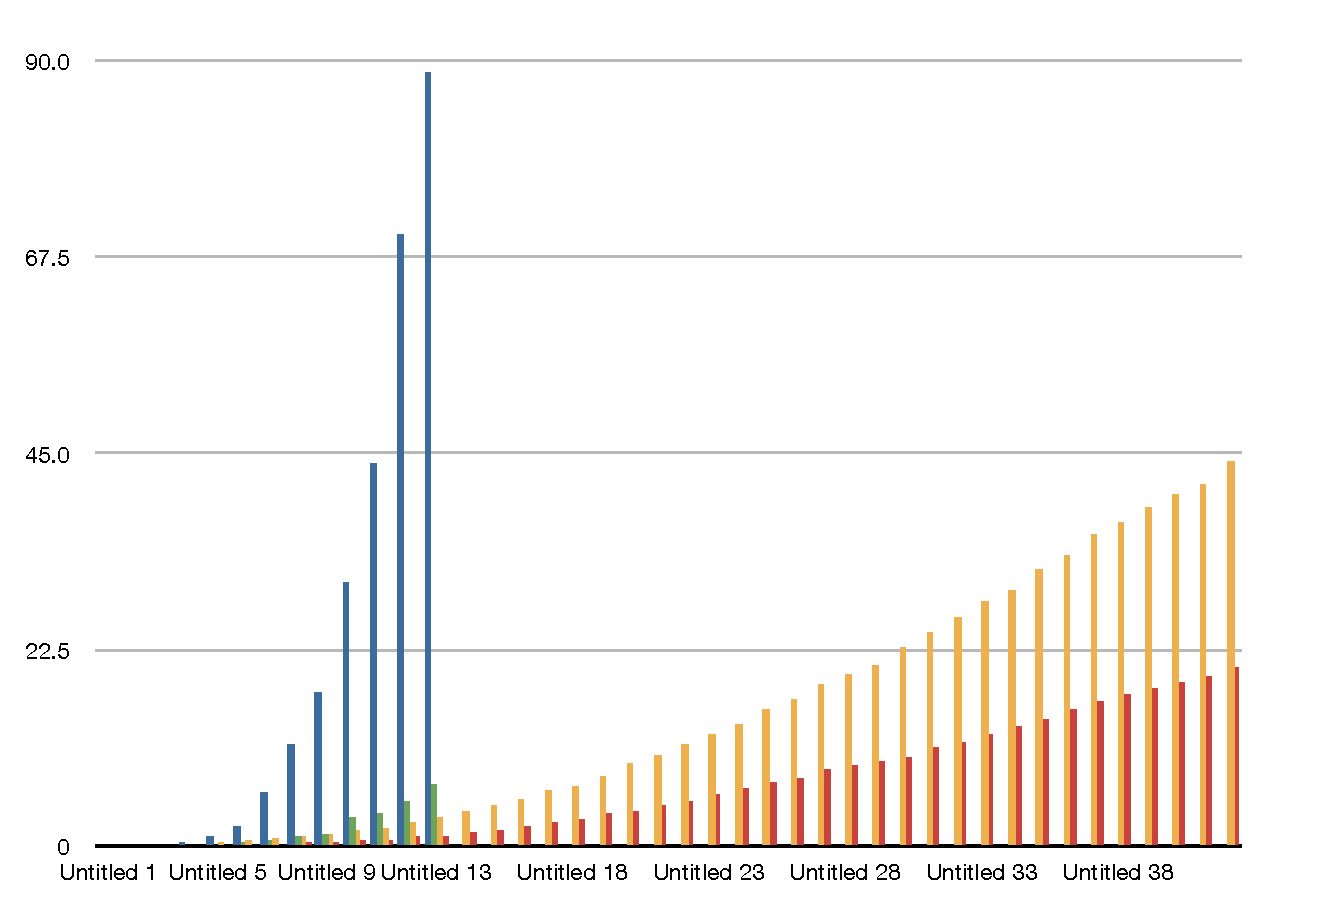
\includegraphics[width=1\columnwidth]{pic-runtime-buttons}
  \caption{Runtimes of FF and SGPLAN on the minimal GIVE worlds for $h=20$. The horizontal axis is $n$, ranging from 1 to 40.}
  \label{fig:give-runtime-minimal}
\end{figure}

\subsection{Experiment 3: GIVE worlds with junk positions}
\label{sec:experiment-3:-give}

Finally, we varied the GIVE world in order to judge the effect of the
universe size in the GIVE domain (see Fig.~\ref{fig:give-junk}).  We
added another $w$ by $h$ positions to the right of a minimal world as
in Experiment 2.  Other than that, we left the initial state and goal
untouched, i.e.\ the new positions were not needed in any plan; this
approximates the situation in the actual GIVE domain, where most grid
positions never need to be used.  As before, we generate a GIVE world
description and then convert it into a planning problem.

\begin{figure}
  \centering
  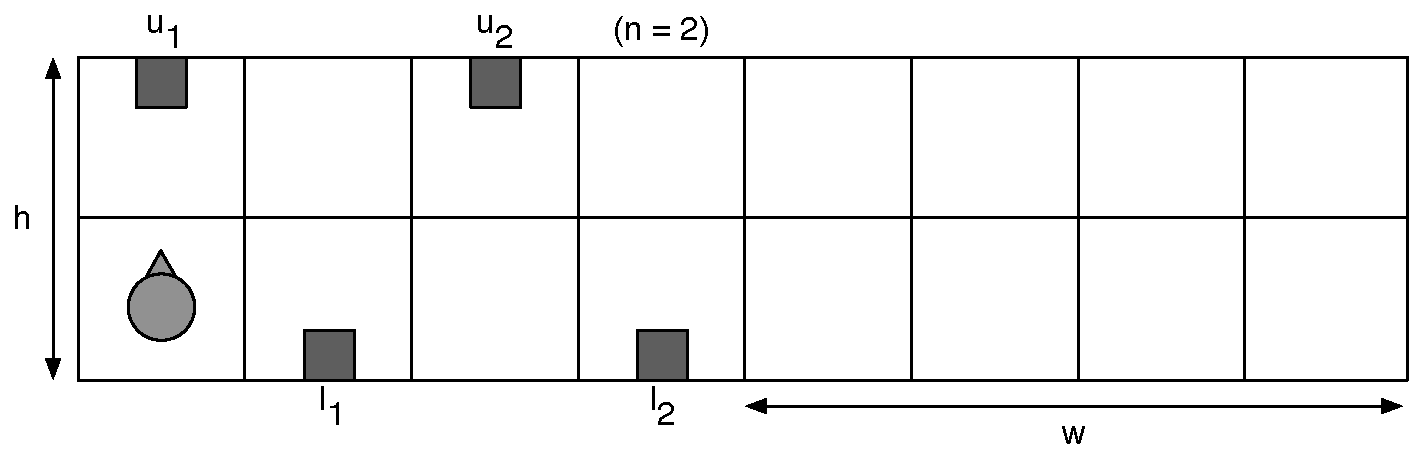
\includegraphics[width=1\columnwidth]{pic-empty-buttons}
  \caption{GIVE world with junk positions.}
  \label{fig:give-junk}
\end{figure}

Some results for $h=20$ and $n=5$ (with $w$ ranging from $1$ to $70$)
are shown in Fig.~\ref{fig:give-runtime-junk}.  Again, FF runs out of
memory, this time at $w=17$, whereas SGPLAN happily solved inputs
beyond $w=70$.  However, unlike in Experiment 2, both planners now
spend a substantial propertion of their time on grounding again.  In
SGPLAN, this translates to a ``parsing time'' (which
\todo{presumably} includes grounding) which grows from 180 ms to 21.7
seconds as $w$ grows from $1$ to $75$; the rest of the runtime (which
includes the search) only grows from 400 ms to 2.3 seconds.  This
difference is particularly dramatic given that the actual optimal plan
is an identical plan of about 100 steps for each $w$.

\begin{figure}
  \centering
  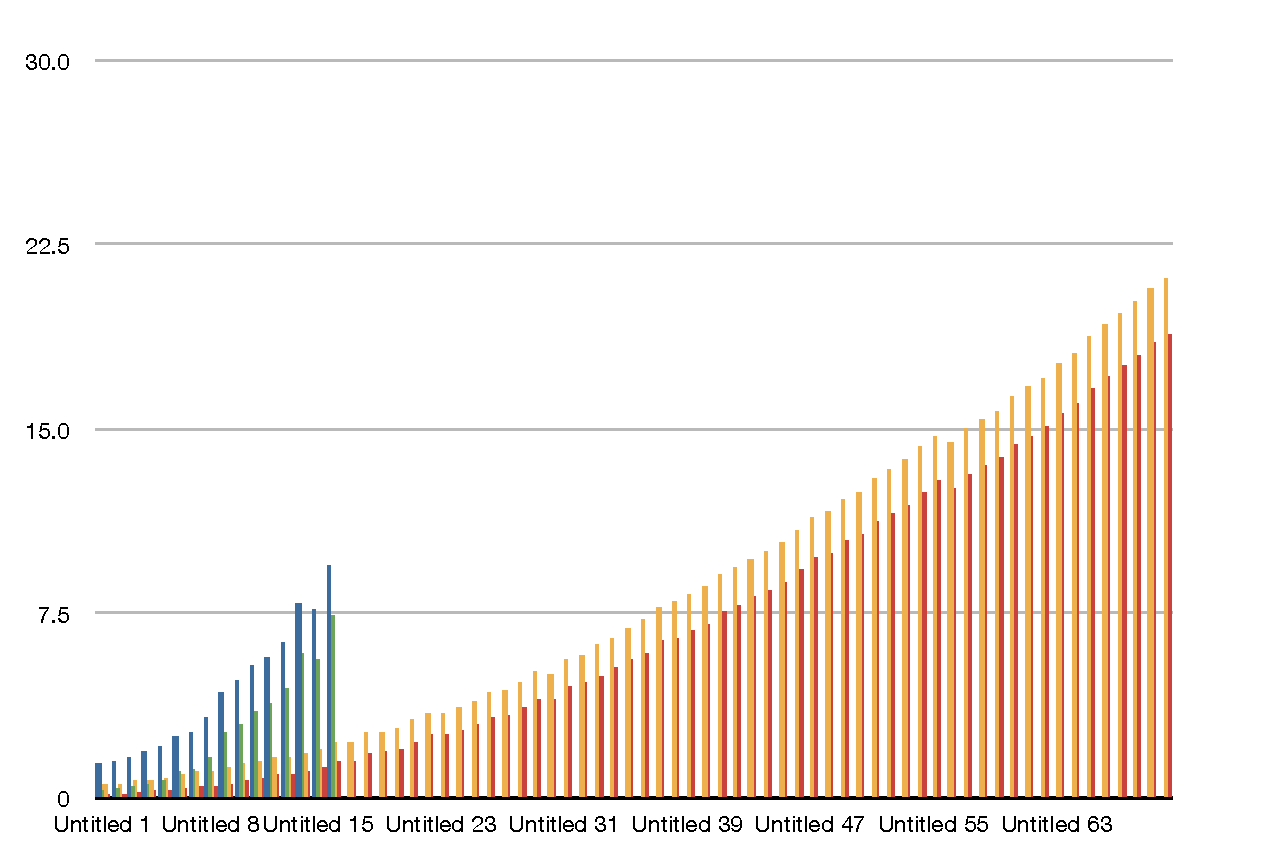
\includegraphics[width=1\columnwidth]{pic-runtime-empty-world}
  \caption{Runtimes of FF and SGPLAN on the GIVE worlds with junk
    positions for $h=20$ and $n=5$. The horizontal axis is $w$,
    ranging from 1 to 70.}
  \label{fig:give-runtime-junk}
\end{figure}


%%% Local Variables: 
%%% mode: latex
%%% TeX-master: "experiences"
%%% End: 
